\documentclass[11pt,a4paper]{article}

\usepackage[T1]{fontenc}
\usepackage[utf8]{inputenc}
\usepackage[margin=1in]{geometry}
\usepackage{amsmath,amssymb,amsthm}
\usepackage{tikz}
\usetikzlibrary{positioning,arrows.meta}
\usepackage{xcolor}
\usepackage{microtype}
\usepackage{hyperref}

\hypersetup{colorlinks=true,linkcolor=blue,citecolor=blue,urlcolor=blue}
\definecolor{accept}{HTML}{1B7837}
\definecolor{reject}{HTML}{C2272D}
\definecolor{neutralg}{HTML}{4D4D4D}

\theoremstyle{plain}
\newtheorem{proposition}{Proposition}

\title{Where the switch cost lives in active inference\\[2pt]
\large Notebook~11's attention rule, decomposed against the EFE formalism}
\author{Internal note --- IWAI 2026 paper}
\date{2026-05-15}

\begin{document}
\maketitle

\begin{abstract}
Notebook~11's deterministic attention rule
``switch iff $\mathrm{EIG}_{\mathrm{best}} > \mathrm{EIG}_{\mathrm{stay}} + c$''
was introduced as an attentional \emph{switch cost}. A forest-walk
discussion asserted that this corresponds to the \emph{pragmatic} term of
expected free energy. \textbf{That assertion is wrong.} The pragmatic
term is a preference over \emph{outcomes}; the switch cost is a cost on
\emph{actions}. This note shows, against the equations of
Da~Costa et~al.~(2020) and Friston et~al.\ (\emph{Active inference and
learning}, 2016), that the switch cost is instead a \emph{policy prior}
$E(\pi)$ --- the habit / control-cost slot of the policy posterior
$\sigma(\ln E - \gamma G)$. Notebook~11's hysteresis rule is precisely
the MAP / winner-take-all action selected from that posterior with flat
outcome preferences and a persistence-favouring habit. The mechanism is
therefore principled in \emph{type}; whether the specific functional
form of $\ln E$ is independently anchored (e.g.\ in attentional
dwell-time data) is a separate, residual question.
\end{abstract}

\section{Lead}

The forest-walk claim was: \emph{the switch cost is the pragmatic term
of EFE that the EIG-only policy was missing}. Reading Da~Costa
et~al.~(2020) carefully, this is wrong. The pragmatic term of $G(\pi)$
is $-\mathbb{E}_{Q(o_\tau\mid\pi)}[\ln P(o_\tau)]$ --- an expectation
over \emph{outcomes} $o_\tau$, weighted by the preference prior
$C \equiv P(o_\tau)$. A switch cost is attached to an \emph{action}; it
is not in the outcome slot.

The honest correction: the switch cost lives in $\ln E(\pi)$, the
\emph{policy prior} (Da~Costa footnote~5; Friston \emph{Active inference
and learning}, Eq.~7). Equivalently, in the optimal-control idiom, it
is a \emph{KL-control cost} for deviating from a default ``stay''
policy. The two pictures in this note --- the anatomy of the policy
posterior (Fig.~\ref{fig:anatomy}) and the hysteresis decision rule
(Fig.~\ref{fig:hysteresis}) --- pin both the location of the slot and
the exact form of the rule.

\section{The expected free energy and where each piece lives}

Da~Costa et~al.~(2020) define the policy posterior (their Eq.~10) as
\begin{equation}
Q(\pi) = \sigma(-G(\pi)),
\label{eq:Qpi}
\end{equation}
with the expected free energy admitting two decompositions of interest.
The \emph{risk + ambiguity} form (their Eq.~13):
\begin{equation}
G(\pi) =
\underbrace{D_{KL}\!\big[Q(s_\tau,A\mid\pi)\,\big\|\,P(s_\tau,A)\big]}_{\text{Risk}}
+
\underbrace{\mathbb{E}_{Q(s_\tau,A\mid\pi)}\!\big[H[P(o_\tau\mid s_\tau,A)]\big]}_{\text{Ambiguity}}.
\label{eq:risk-ambiguity}
\end{equation}
And the \emph{value} decomposition (their Eq.~16):
\begin{align}
G(\pi) =\;{}&
- \underbrace{\mathbb{E}_{Q(o_\tau\mid\pi)}[\ln P(o_\tau)]}_{\text{Extrinsic / pragmatic}} \notag\\
& - \underbrace{\mathbb{E}_{Q(o_\tau\mid\pi)}\!\big[D_{KL}[Q(s_\tau\mid o_\tau,\pi)\,\|\,Q(s_\tau\mid\pi)]\big]}_{\text{Salience (info gain about states)}} \notag\\
& - \underbrace{\mathbb{E}_{Q(o_\tau,s_\tau\mid\pi)}\!\big[D_{KL}[Q(A\mid o_\tau,s_\tau,\pi)\,\|\,Q(A)]\big]}_{\text{Novelty (info gain about parameters)}}
\;-\; (\text{evidence bound}).
\label{eq:value-decomp}
\end{align}

Two readings off Eq.~\eqref{eq:value-decomp}.

\paragraph{The pragmatic term is over outcomes.}
$-\mathbb{E}_{Q(o_\tau\mid\pi)}[\ln P(o_\tau)]$ is an expectation under
the predicted-outcome distribution, weighted by $C \equiv P(o_\tau)$.
The review text is unambiguous: ``higher-valued \emph{outcomes} have
higher prior probability under $P(o)$ reflecting agent preferences ---
\textbf{not costs on actions themselves}.''

\paragraph{Notebook~11's EIG \emph{is} the novelty term.}
$\mathbb{E}\big[D_{KL}[Q(A\mid o,s,\pi)\,\|\,Q(A)]\big]$ is the expected
information gain about a model \emph{parameter}. The closed-form
$\tfrac12\log\det(\Lambda + hh^\top/\sigma^2) - \tfrac12\log\det(\Lambda)$
implemented by \texttt{expected\_info\_gain\_vec} is exactly that
quantity for the linear-Gaussian model over $\theta$. Da~Costa: ``\emph{It
is this term that underwrites artificial curiosity \dots maximising
intrinsic value corresponds to optimal Bayesian design.}'' So one half
of nb11's policy is principled and correctly named.

\section{Anatomy of the policy posterior}

The full policy posterior, with the prior over policies made explicit,
is given by Friston et~al.\ (\emph{Active inference and learning},
Eq.~7):
\begin{equation}
Q(\pi) = \sigma\big(\ln E(\pi) \,-\, \gamma\, G(\pi)\big).
\label{eq:Qpi-full}
\end{equation}
Da~Costa's footnote~5 confirms the same structure: ``\emph{A more
complete treatment may include priors over policies --- usually denoted
by $E$ \dots leading to an approximate posterior of the form
$\sigma(-\ln E - F - G)$.}'' Friston: ``\emph{$E(\pi)$ \dots creates an
implicit cost structure through prior preferences rather than explicit
penalties},'' with a designated \emph{habitual} policy that the prior
can favour. This is the slot a cost-for-deviating-from-a-default-policy
lives in.

Figure~\ref{fig:anatomy} pins each of nb11's pieces to its location in
that anatomy.

\begin{figure}[h]
\centering
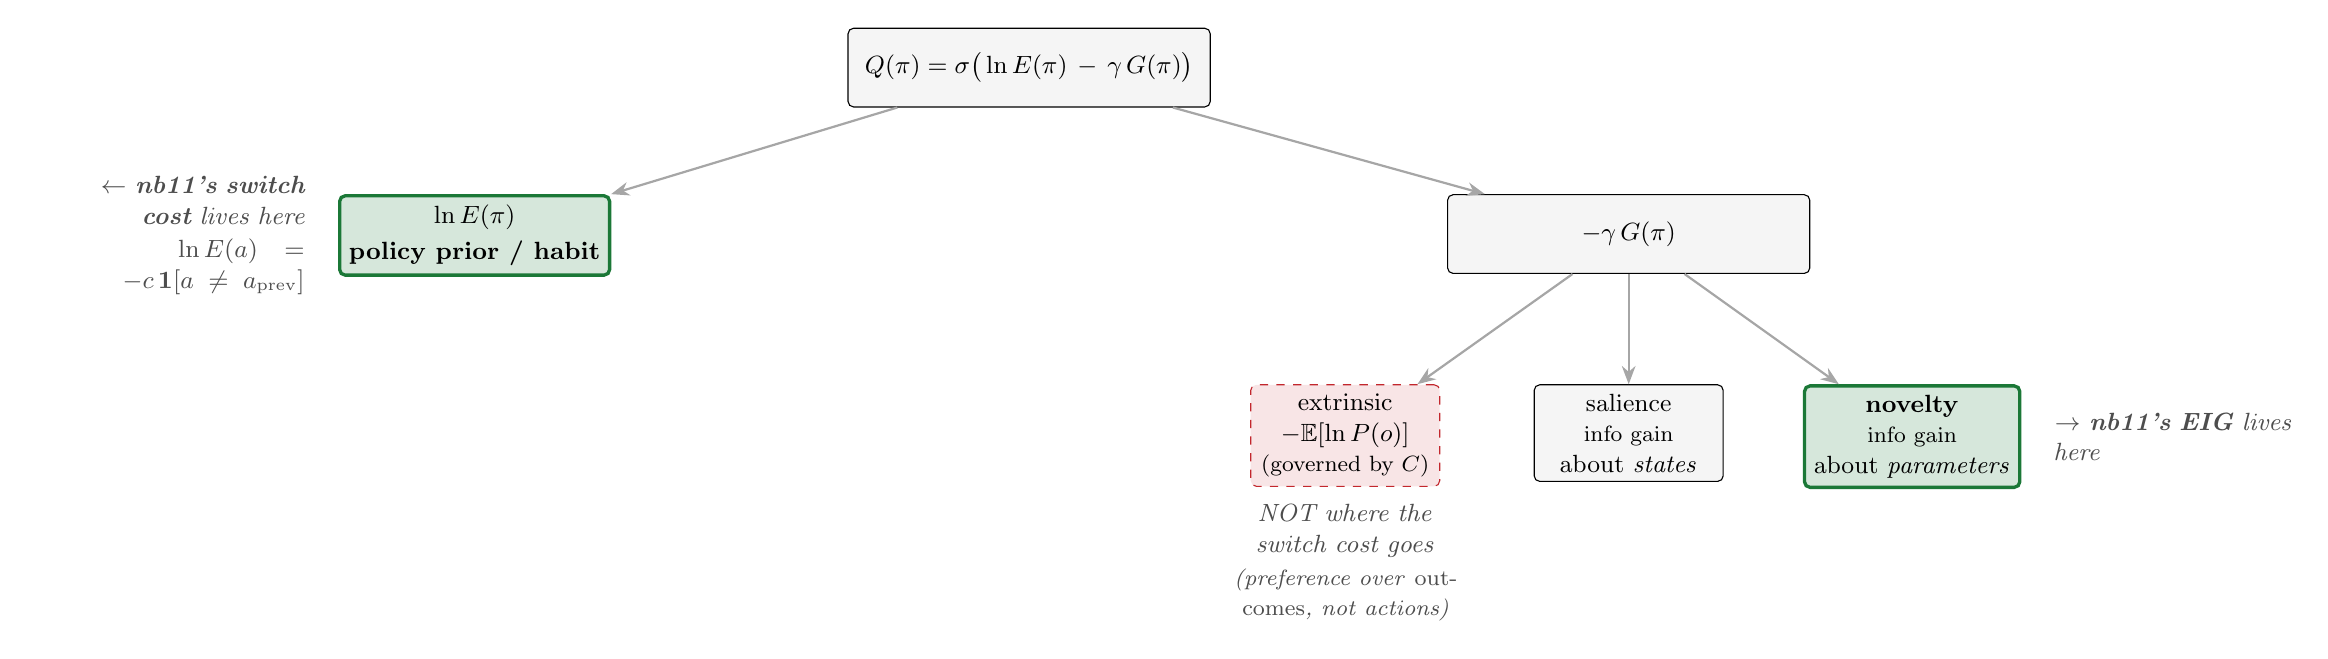
\begin{tikzpicture}[
    node distance=11mm and 16mm,
    box/.style={draw, rounded corners=2pt, minimum height=10mm, minimum width=24mm, align=center, font=\small},
    eq/.style={box, fill=gray!8, minimum width=46mm},
    here/.style={box, fill=accept!18, very thick, draw=accept},
    nothere/.style={box, fill=reject!12, dashed, draw=reject},
    annot/.style={font=\small\itshape, color=neutralg},
    arr/.style={->, >=Stealth, thick, gray!70}
]
  \node[eq] (Q) {$Q(\pi) = \sigma\big(\ln E(\pi) \,-\, \gamma\, G(\pi)\big)$};
  \node[here, below left=of Q, xshift=-14mm] (E) {$\ln E(\pi)$\\[2pt]\textbf{policy prior / habit}};
  \node[eq, below right=of Q, xshift=14mm] (G) {$-\gamma\, G(\pi)$};
  \draw[arr] (Q) -- (E);
  \draw[arr] (Q) -- (G);

  \node[nothere, below=14mm of G, xshift=-36mm] (Ext) {extrinsic\\$-\mathbb{E}[\ln P(o)]$\\\footnotesize (governed by $C$)};
  \node[box, fill=gray!8, below=14mm of G, xshift=0mm] (Sal) {salience\\\footnotesize info gain\\about \emph{states}};
  \node[here, below=14mm of G, xshift=36mm] (Nov) {\textbf{novelty}\\\footnotesize info gain\\about \emph{parameters}};
  \draw[arr] (G) -- (Ext);
  \draw[arr] (G) -- (Sal);
  \draw[arr] (G) -- (Nov);

  \node[annot, left=3mm of E, text width=34mm, align=right]
       {$\leftarrow$ \textbf{nb11's switch cost} lives here\\[1pt]
        $\ln E(a) = -c\,\mathbf{1}[a\!\neq\! a_{\mathrm{prev}}]$};
  \node[annot, right=3mm of Nov, text width=30mm, align=left]
       {$\rightarrow$ \textbf{nb11's EIG} lives here};
  \node[annot, below=1mm of Ext, text width=44mm, align=center]
       {NOT where the switch cost goes\\[1pt]
        \footnotesize (preference over \emph{outcomes}, not actions)};
\end{tikzpicture}
\caption{Anatomy of the active-inference policy posterior, with
notebook~11's two ingredients pinned to their slots. The switch cost
sits in the \textbf{policy prior $E(\pi)$} (green, top-left), \emph{not}
in the extrinsic / pragmatic value (red, bottom-left). The EIG is the
\textbf{novelty} term of $-G(\pi)$ (green, bottom-right).}
\label{fig:anatomy}
\end{figure}

\section{Why the switch cost is not the pragmatic term}

A switch cost is attached to an \emph{action} (switching attention).
The pragmatic term is an expectation over \emph{outcomes}
(Eq.~\eqref{eq:value-decomp}). There is no construal under the standard
discrete-state EFE in which ``penalise the switch action'' becomes
$-\mathbb{E}[\ln P(o_\tau)]$. The forest-walk identification was a
type-error.

\section{Where it actually lives: the policy prior $E(\pi)$}

The policy posterior~\eqref{eq:Qpi-full} contains an additive
$\ln E(\pi)$ term that does not depend on $G(\pi)$ at all. Setting
\begin{equation}
\ln E(a) \;=\; -\,c \cdot \mathbf{1}[\,a \neq a_{\mathrm{prev}}\,]
\label{eq:logE}
\end{equation}
is a log-policy-prior that favours the persistence / habitual policy by
a fixed log-odds ratio $c$ relative to any deviation. This is the
standard ``habit'' form (Friston, \emph{Active inference and learning},
\S2).

\section{Equivalence: nb11's rule is MAP under the policy posterior}

Notebook~11's deterministic attention rule is, with $c$ for the switch
cost,
\begin{equation*}
a_t = \begin{cases}
\arg\max_a \mathrm{EIG}_a & \text{if } \max_a\mathrm{EIG}_a > \mathrm{EIG}_{a_{\mathrm{prev}}} + c,\\
a_{\mathrm{prev}} & \text{otherwise.}
\end{cases}
\end{equation*}

\begin{proposition}
Let $V(a) := \mathrm{EIG}_a - c\,\mathbf{1}[a\neq a_{\mathrm{prev}}]$
with $c>0$. Then $a_t = \arg\max_a V(a)$, and equivalently $a_t$ is the
MAP action under the active-inference policy
posterior~\eqref{eq:Qpi-full} with novelty $\mathrm{EIG}_a$, flat
outcome preferences (extrinsic value constant in $a$, so
$-\gamma G(a) = \gamma\,\mathrm{EIG}_a + \text{const}$), EFE precision
$\gamma=1$, and policy prior~\eqref{eq:logE}. In the high-precision
limit (Da~Costa~\S6.3), the softmax collapses to argmax, so the
deterministic rule is exactly this MAP.
\end{proposition}

\begin{proof}
Let $M = \max_{a\neq a_{\mathrm{prev}}} \mathrm{EIG}_a$ and
$S = \mathrm{EIG}_{a_{\mathrm{prev}}}$. From~\eqref{eq:logE},
$V(a_{\mathrm{prev}}) = S$ and $V(a) = \mathrm{EIG}_a - c$ for
$a\neq a_{\mathrm{prev}}$. Thus $\arg\max_a V(a) = a_{\mathrm{prev}}$
iff $S \geq M-c$, i.e.\ iff $M \leq S + c$; otherwise
$\arg\max_a V(a) = \arg\max_{a\neq a_{\mathrm{prev}}}\mathrm{EIG}_a$.

Now compare to nb11's rule. Let $B = \max_a \mathrm{EIG}_a$.
\emph{Case A:} the global argmax is $a_{\mathrm{prev}}$, so $B = S$.
Then $B > S + c$ is false ($c > 0$), so nb11 stays. And
$M \leq S \leq S + c$, so $V$-argmax also stays.
\emph{Case B:} the global argmax is some
$a^\ast \neq a_{\mathrm{prev}}$, so $B = M$. Both rules switch iff
$M > S+c$, and both then go to
$\arg\max_{a\neq a_{\mathrm{prev}}}\mathrm{EIG}_a = a^\ast$. \qedhere
\end{proof}

Figure~\ref{fig:hysteresis} visualises the rule on three bands.

\begin{figure}[h]
\centering
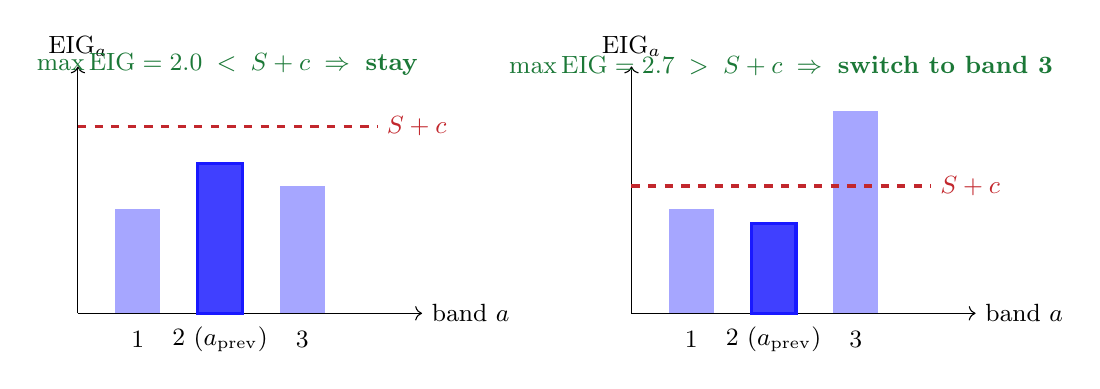
\begin{tikzpicture}[scale=0.95, every node/.style={font=\small}]

% --- Scenario A: stay wins ---
\begin{scope}
  \draw[->] (0,0) -- (4.6,0) node[right] {band $a$};
  \draw[->] (0,0) -- (0,3.3) node[above] {$\mathrm{EIG}_a$};
  \fill[blue!35] (0.5,0) rectangle (1.1,1.4);
  \fill[blue!75, draw=blue!90, very thick] (1.6,0) rectangle (2.2,2.0);
  \fill[blue!35] (2.7,0) rectangle (3.3,1.7);
  \node at (0.8,-0.35) {1};
  \node at (1.9,-0.35) {2 ($a_{\mathrm{prev}}$)};
  \node at (3.0,-0.35) {3};
  \draw[reject, dashed, very thick] (0,2.5) -- (4.0,2.5);
  \node[reject, anchor=west] at (4.0,2.5) {$S + c$};
  \node[anchor=south, accept] at (2.0,3.05)
       {$\max\mathrm{EIG}=2.0 \;<\; S+c \;\Rightarrow\;$ \textbf{stay}};
\end{scope}

% --- Scenario B: switch wins ---
\begin{scope}[xshift=7.4cm]
  \draw[->] (0,0) -- (4.6,0) node[right] {band $a$};
  \draw[->] (0,0) -- (0,3.3) node[above] {$\mathrm{EIG}_a$};
  \fill[blue!35] (0.5,0) rectangle (1.1,1.4);
  \fill[blue!75, draw=blue!90, very thick] (1.6,0) rectangle (2.2,1.2);
  \fill[blue!35] (2.7,0) rectangle (3.3,2.7);
  \node at (0.8,-0.35) {1};
  \node at (1.9,-0.35) {2 ($a_{\mathrm{prev}}$)};
  \node at (3.0,-0.35) {3};
  \draw[reject, dashed, very thick] (0,1.7) -- (4.0,1.7);
  \node[reject, anchor=west] at (4.0,1.7) {$S + c$};
  \node[anchor=south, accept] at (2.0,3.05)
       {$\max\mathrm{EIG}=2.7 \;>\; S+c \;\Rightarrow\;$ \textbf{switch to band 3}};
\end{scope}

\end{tikzpicture}
\caption{The hysteresis rule visualised. Bars show the three bands'
$\mathrm{EIG}_a$; the highlighted bar is the current band
($a_{\mathrm{prev}}$, with value $S$); the red dashed line is the
switching threshold $S + c$. Equivalently, the agent picks
$\arg\max_a [\mathrm{EIG}_a - c\,\mathbf{1}[a\neq a_{\mathrm{prev}}]]$
--- the persistence default gets a free pass; every other option pays a
tax of $c$.}
\label{fig:hysteresis}
\end{figure}

\section{The KL-control reading}

Da~Costa's text under Eq.~\eqref{eq:risk-ambiguity}: ``\emph{In the
optimal control literature, this form of expected free energy
underwrites \textbf{KL control}}'' (Todorov~2009; Kappen, G\'omez \&
Opper~2012). KL control parametrises the cost of a controlled policy as
a KL divergence from a \emph{passive / default} policy ---
mathematically the same slot as $\ln E(\pi)$. Notebook~11's
$\mathbf{1}[a \neq a_{\mathrm{prev}}]$ with default ``stay'' is exactly
a discrete, hard-threshold control cost on deviation from the passive
policy. Whether one names it ``policy prior,'' ``habit,'' or
``KL-control cost'' is a matter of register; the formal object is one
and the same.

\section{Honest bottom line}

\begin{itemize}
\item \textbf{Principled in \emph{type} --- yes.} The switch cost
populates a standard, named slot in the active-inference policy
posterior: the policy prior $E(\pi)$ / habit / KL-control cost. It sits
additively beside $-\gamma G(\pi)$. nb11's hysteresis rule is exactly
the MAP action under that posterior with flat preferences and a
persistence-favouring habit (Proposition~1). The forest-walk worry that
the mechanism is \emph{ad hoc} machinery is not borne out: the EIG-only
policy was simply missing the $E(\pi)$ term, and the switch cost is the
(MAP limit of) it.

\item \textbf{Principled in \emph{form and value} --- not
automatically.} The formalism \emph{permits} a policy prior; it does not
\emph{dictate} the flat additive form $\ln E(a) = -c\,\mathbf{1}[a\neq
a_{\mathrm{prev}}]$ or any particular value of $c$. Choosing the
simplest possible form, and tuning $c$ until the network oscillated,
remain researcher degrees of freedom. The framework legitimises the
\emph{slot}; it does not absolve the \emph{choice}. The straightforward
fix: anchor $c$ in attentional dwell-time / task-switching-cost
literature (Monsell; Duncan, Ward \& Shapiro), so what was a free
parameter becomes either a prediction or a measurement-driven
constraint.

\item \textbf{One footnote, for completeness.} In the strong
active-inference claim that ``there are no cost functions, only
priors,'' action / effort costs get reified as proprioceptive
\emph{outcome} preferences and folded back into $C$. Under that reading
the forest walk could be partially salvaged --- but the standard
discrete-state formulation (Da~Costa) puts the cost in $E(\pi)$, and
that is the cleaner home for nb11.
\end{itemize}

\paragraph{For nb11.} Recast the parameter from \texttt{switch\_cost}
to ``persistence policy prior'' with the equation
$\ln E(a) = -c\,\mathbf{1}[a\neq a_{\mathrm{prev}}]$, cite Da~Costa
footnote~5 and Friston \emph{Active inference and learning} for the
slot, cite the KL-control lineage for the form, and state plainly that
the form is the simplest choice and the value should ideally be
anchored to dwell-time data. This is both correct and a stronger
framing than ``we added a switch cost.''

\begin{thebibliography}{9}

\bibitem{daCosta2020}
L.~Da~Costa, T.~Parr, N.~Sajid, S.~Veselic, V.~Neacsu, K.~Friston (2020).
\emph{Active inference on discrete state-spaces: a synthesis.}
Journal of Mathematical Psychology, 99:102447.
\href{https://arxiv.org/abs/2001.07203}{arXiv:2001.07203}.

\bibitem{Friston2016learning}
K.~Friston, T.~FitzGerald, F.~Rigoli, P.~Schwartenbeck, J.~O'Doherty,
G.~Pezzulo (2016).
\emph{Active inference and learning.}
Neuroscience and Biobehavioral Reviews 68:862--879.
\href{https://pmc.ncbi.nlm.nih.gov/articles/PMC5167251/}{PMC5167251}.

\bibitem{Friston2015epistemic}
K.~Friston, F.~Rigoli, D.~Ognibene, C.~Mathys, T.~FitzGerald,
G.~Pezzulo (2015).
\emph{Active inference and epistemic value.}
Cognitive Neuroscience 6(4):187--214.

\bibitem{ParrFriston2019}
T.~Parr, K.~Friston (2019).
\emph{Generalised free energy and active inference.}
Biological Cybernetics 113:495--513.
\href{https://pmc.ncbi.nlm.nih.gov/articles/PMC6848054/}{PMC6848054}.

\bibitem{Todorov2009}
E.~Todorov (2009).
\emph{Efficient computation of optimal actions.}
PNAS 106(28):11478--11483.

\bibitem{KappenGomezOpper2012}
H.~J.~Kappen, V.~G\'omez, M.~Opper (2012).
\emph{Optimal control as a graphical model inference problem.}
Machine Learning 87:159--182.

\bibitem{Levine2018}
S.~Levine (2018).
\emph{Reinforcement learning and control as probabilistic inference:
tutorial and review.}
\href{https://arxiv.org/abs/1805.00909}{arXiv:1805.00909}.

\end{thebibliography}

\end{document}
